\section{Data Rate}


\ac{GI} and \ac{CR}
\begin{figure}%
	\centering
	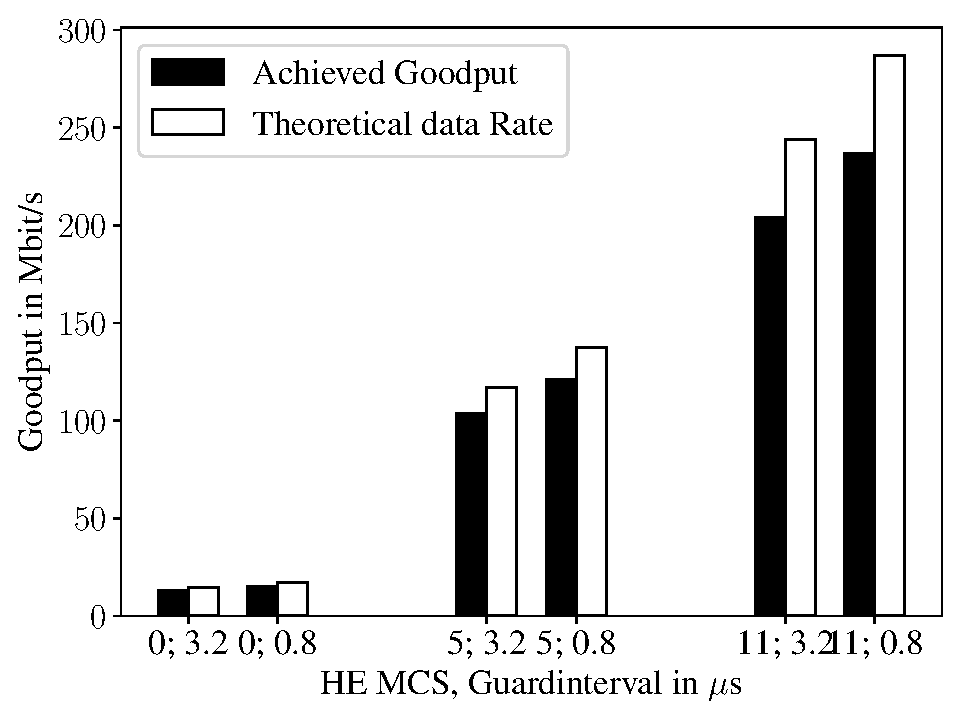
\includegraphics[width=0.95\textwidth]{figures/gi_dataRate_simulation.pdf}
	\caption{Achieved Goodput and theoretical Datarate of two WiFi 6 stations in Ad-Hoc Mode with \num{2} \ac{MIMO} streams and a bandwidth of \SI{80}{\mega\hertz} in regards to the number of \ac{MIMO} streams and the chosen \ac{MCS} and \ac{CR}}%
	\label{fig:Data_rate_GI}%
\end{figure}

atteninuation of bandwidth : 800ns : \SI{94}{\percent} \SI{89}{\percent} \SI{80}{\percent}

Factors apply for MCS0 but may also apply later

\begin{figure}%
	\centering
	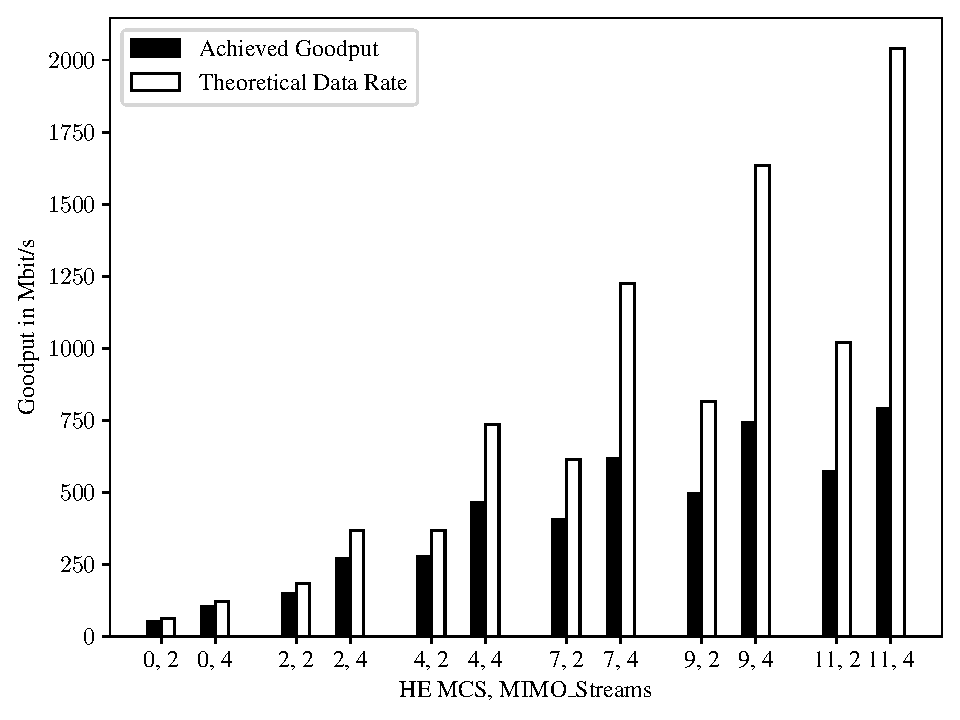
\includegraphics[width=0.95\textwidth]{figures/mimo_dataRate_simulation.pdf}
	\caption{Achieved Goodput and theoretical Datarate of two WiFi 6 stations in Ad-Hoc Mode with a \ac{GI} of \SI{3200}{\nano\second} and a bandwidth of \SI{80}{\mega\hertz} in regards to the number of \ac{MIMO} streams and the chosen \ac{MCS} and \ac{CR}}%
	\label{fig:Data_rate_Mimo}%
\end{figure}


\begin{figure}%
	\centering
	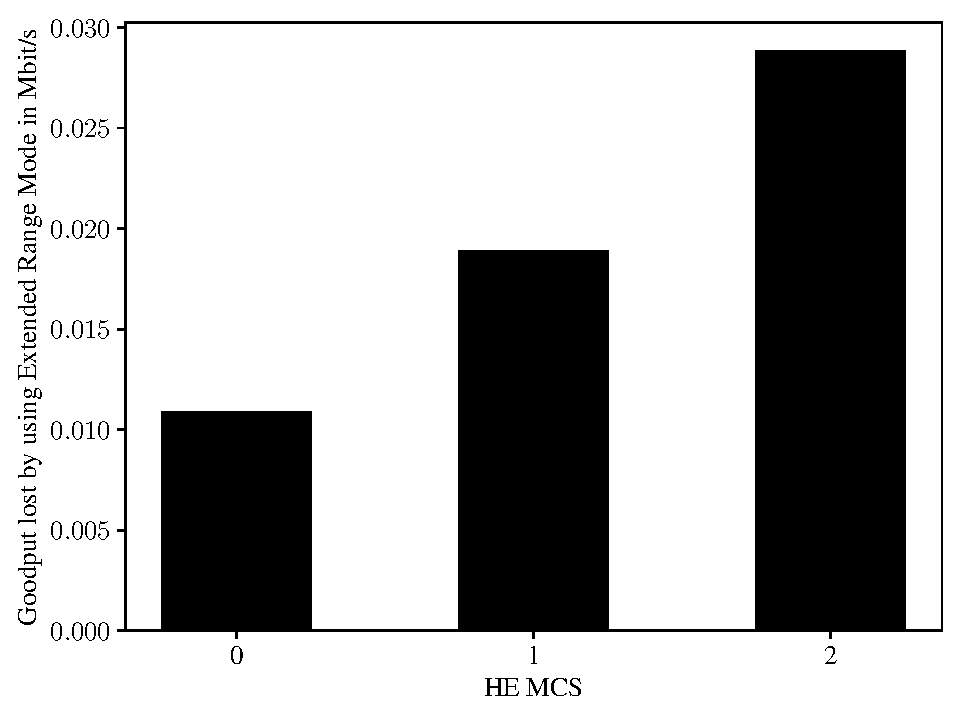
\includegraphics[width=0.95\textwidth]{figures/ER_dataRate_simulation.pdf}
	\caption{Achieved Goodput and theoretical Datarate of two WiFi 6 stations in Ad-Hoc Mode with a \ac{GI} of \SI{3200}{\nano\second} and a bandwidth of \SI{20}{\mega\hertz} in regards to the number of \ac{MIMO} streams and the chosen \ac{MCS} and \ac{CR}}%
	\label{fig:Data_rate_ER}%
\end{figure}

\todo{DataRate for STBC}
STBC and DCM * 2 payload / half data rate

\begin{figure}%
	\centering
	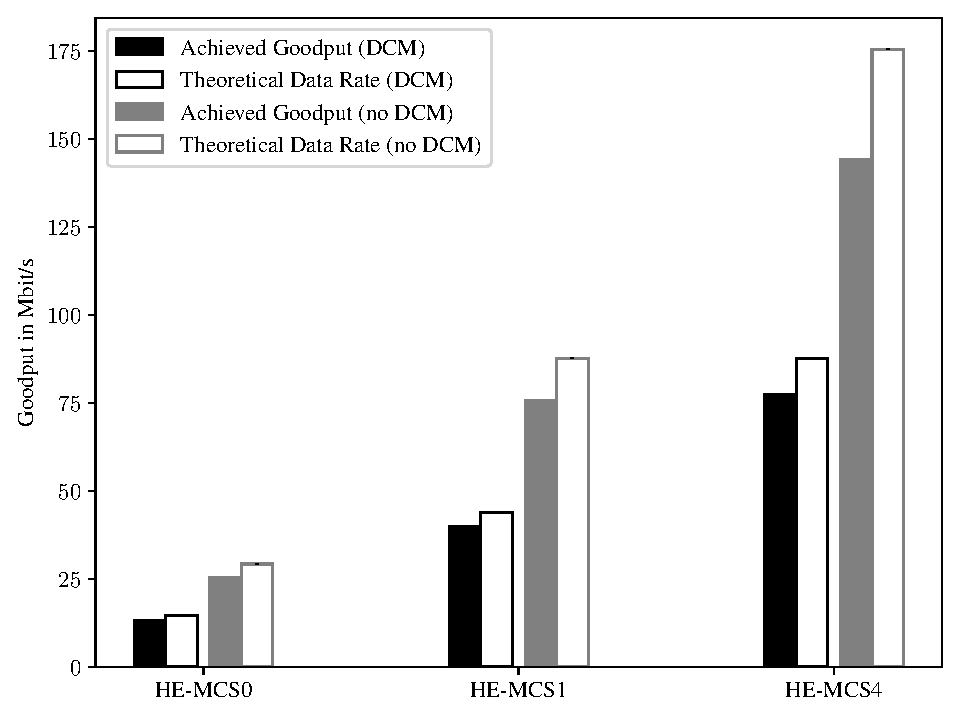
\includegraphics[width=0.95\textwidth]{figures/DCM_dataRate_simulation.pdf}
	\caption{Achieved Goodput and theoretical Datarate of two WiFi 6 stations in Ad-Hoc Mode with for IEEE 802.11ax physical layer parameters of a \ac{GI} of \SI{3200}{\nano\second}, a \ac{BW} of \SI{40}{\mega\hertz} and 2 spatial streams  in regards to the number of the chosen HE-\ac{MCS} value and whether \ac{DCM} is enabled}%
	\label{fig:Data_rate_DCM}%
\end{figure}


But Latency?
Latency is always based on Data Rate and Robustness

Data Rate and Robustness als related to oneanother

